%!TEX root = ../article.tex

% \listoftodos

%1
\levelA{\label{chap:introduction}Introduction}
\input{content/1-introduction.tex}
    %\levelB{Motivation}
    %from pep 1, paragrafo 1
In a forensic context, file recovery is a frequent task that can be motivated by several situations, like physical media malfunction, intentional attempt to hide data, and the need to access deleted or older versions of files. When the filesystem no longer provides the physical location of a file on the media, data carving is often the only procedure capable of retrieving this content.

%from pep 1, paragrafo 2
Data carving is a forensic process that attempts to recover files without previous information of where the file starts or ends \cite{garfinkel_carving_2007}.
To accomplish this, a program has to analyze a source of raw data, searching for patterns indicating a known file type and making attempts to locate and reconstruct each of its constituent parts.

%from pep 1, paragrafo 2b
That process commonly disregards the filesystem \cite{veenman_statistical_2007}, being able to recover deleted files from unallocated areas, but faces the problem of fragmentation \cite{veenman_statistical_2007}  \cite{pal_evolution_2009}: in many cases, files are not written sequentially on disk and deleted files may have missing parts.

This procedure is frequently used in forensic environments, but it may also be beneficial in other areas, such as reverse engineering, network traffic analysis, and data mining.

This observation is related to the fact that many types of data sources contain embedded files. Therefore, they may be used as input to a data carving process. This includes network traffic, memory dumps, hard drive images, and files containing other files.

    
\subsection{Example}
% \todo[color=gray,inline]{deixar ou tirar fora?}

Normally, the average user of a computer does not need to deal with hard disk sectors directly and has contact only with the already mounted filesystem, which presents directories and files for the user. But to present such a view, the operating system has to interpret the raw media data, which is simply a stream of data blocks.

To explain how a data carving process works, a hard drive with a deleted video file is here used as an example.
The first blocks of the drive contain a partition table, indicating ranges of blocks belonging to each of the drive partitions. Inside a partition, the operating system expects to find a filesystem. The filesystem stores metadata about each file or directory and keeps an index indicating the position of each file on disk. This way, when a user opens a file, the operating system uses the filesystem to find where in the disk the file is stored, accessing those areas directly and returning its content to the user, who sees the returned data as the file content. 
 
If the video file in the example had not been deleted, the filesystem could use the index to find the video location on disk. But after deletion, the corresponding index entry is erased, while the actual content of the file may be left untouched to avoid disk access. In this circumstance, a data carving procedure may successfully retrieve the file, even if the filesystem cannot. One common data carving approach that does not deal with fragmentation consists of searching for headers and footers patterns. To retrieve the hypothetical video file in the example, a software using this approach would sequentially read each drive sector, find a known header of a video file and save the following sectors until a footer is found or a size limit is reached. 

    %  \subsection{Data carving categorization}
%  \todo[color=gray,inline]{será que todas essas classificações não confundem mais do que explicam? não tenho certeza}
 

%from pep 2.2, paragrafo 1
Ali et al. \cite{ali_review_2018} divide the data carving process into three steps:
    identification, which classifies the file type of individual chunks of data; 
    validation, which includes a list of requirements of a file that are needed for its recovery to be considered successful; and
    reassembling, which attempts to reconstruct the original file.
    

%from pep 2.2, paragrafo 3
Nadeem \cite{nadeem_ashraf_forensic_2013} groups the carving techniques in three generations, each extending the previous one.
%from pep 2.2, paragrafo 4
The first generation is header-footer based carving. It uses file signatures like magic-bytes, headers, and footers to identify the beginning and end of a file.
%from pep 2.2, paragrafo 5
The second generation is structure-based carving, also called ``semantic carving'' or ``deep carving''. It reduces the number of false positives by using file structure knowledge to perform validation.
%from pep 2.2, paragrafo 6
The third generation advances reassembling with methods to deal with fragmentation. It tries to infer relationships and order between chunks of data based on content and statistical analysis to reassemble the original file.

%from pep 2.2, paragrafo 7
For file type detection, which could be mapped to the identification step in the  process steps of Ali et al. \cite{ali_review_2018}, Amirami et al. \cite{amirani_new_2008} cite three categories: extension-based identification, magic bytes-based identification, and content-based identification.
In extension-based identification, the content of the file is ignored and only its filename extension is used. Magic bytes-based identification uses signatures, generally a fixed string, usually at the beginning of a file. It is a common strategy that uses header/footer, but not all files adopt it. Content-based identification identifies the file using some statistical modeling of its content.

%from pep 2.2, paragrafo 8
Beebe et al. \cite{beebe_sceadan:_2013} identify three content-based approaches to classify file and data types, also referring only to the identification step of the Ali et al. \cite{ali_review_2018} data carving process division: semantic parsing, nonsemantic parsing, and machine learning. Semantic parsing relies on the file structure to identify its type. Nonsemantic parsing searches for strings that are commonly found in specific files. Machine learning uses supervised and unsupervised algorithms, like Support Vector Machine (SVM), k-Nearest Neighbors (kNN), and Neural Networks (NN).

\sigla{NN}{Neural Networks}
\sigla{kNN}{k-Nearest Neighbors}
\sigla{SVM}{Support Vector Machine}

%from pep 2.2, paragrafo 9
A summary of the categorization schemes is depicted in Table \ref{tab:categories}. As Nadeem \cite{nadeem_ashraf_forensic_2013} does not specifically mention machine learning, it is left out of generation classification.

\begin{table*}[!ht]
    \centering
    \caption{Summary of data carving categorization schemes according to other authors}
    \label{tab:categories}
    \begin{tabular}{ l | l | l | c }
      Steps & \multicolumn{2}{|c|}{Techniques}                  & Generation\\
      \hline\hline
      Identification    & extension-based   &                   &   \\
                        \cline{2-3}
                        & magic bytes-based &                   & \multirow{-2}{*}{1\textsuperscript{st}}\\
                        \cline{2-4}
                        & content-based     & semantic          &   \\
                                            \cline{3-3}
                        &                   & non-semantic      & \multirow{-2}{*}{2\textsuperscript{nd}}\\
                                            \cline{3-4}
                        &                   & machine learning  &  --- \\
      \hline
      Validation        &                   &                   & 2\textsuperscript{nd} \\
      \hline
      Reassembling      &                   &                   & 3\textsuperscript{rd}\\
      \hline
    \end{tabular}
\end{table*}



    %\subsection{The problem}
% the problem of data carving development
%from pep 1, paragrafo 4
Although there are researches providing good alternatives in data carving, the algorithms used in practice by available data carving software are generally still manually coded, using fixed byte sequences found on headers and footers of the files. The amount of different file types combined with the slow process of manually coding each of those patterns makes the development of data carving software an overwhelming task \cite{mcdaniel_content_2003}. 

% ml as a solution
%from pep 1, paragrafo 5
% The application of machine learning solutions to this manual task has the potential to make it easier and faster. An initial strategy could be to train a classifier to, given a chunk of data, provide a label indicating a file type. That could be used to recover unfragmented deleted files.
% % novo
% Then, that same classifier can be applied in small chunks of data to produce input to a second algorithm, responsible to reassemble the fragments of a file.

% ml as a solution
%from pep 1, paragrafo 6
% The recovery of fragmented files through data carving would require some sort of pattern recognition on the identified chunks, in order to reconstruct the correct sequence.

%from pep 4, paragrafo 3
The amount of work required to support the vast amount of file types in existence is arguably the main obstacle to implement new technologies on data carving software. The forensic community would benefit from researches that could make the task of supporting the carving of a new file type easier. Machine learning techniques have the potential to achieve that goal because they can replace the step of manually encoding a structure parser by automatically recognizing patterns in large amounts of data.

The range of common file types, files that are most likely to be relevant in a piece of evidence, like images, videos, and documents, do not change frequently. Because of that, the available tools could so far be kept up to date, despite the work required to include a new file type.

But there are situations when this is not enough. This can happen when the relevant file type is proprietary, uncommon, or newly created. As an example, some video surveillance solutions use proprietary video formats that are not recognized by data carving software. In this situation, it would be beneficial to use a tool that, using examples of files of that particular kind, could create a customized model able to identify and retrieve this file type.

One strategy to solve this problem could be the use of Neural Networks \cite{} to provide automatic classification of file fragments. As detailed in section \ref{sec:relatedwork}, some works already explored the use of Neural Networks to perform file fragment classification. But the practice of using the file extension as labels for each of the file fragments may introduce errors when multiple file types use the same data structures. Thus, the plain search for better models without tackling the problem of inner data labeling may not be enough to achieve higher accuracy results.
    %\levelB{Research questions}
    %\subsection{Research question}
% This work compares the use of Multilayer Perceptrons (MLP), Convolutional Neural Networks (CNN) and Long Short-Term Memory (LSTM), and combinations of those types of networks, to perform file fragment classification, which is the first step of the data carving process, identification, answering the following initial questions:
The main goal of this paper is to identify which models of Neural Network would provide the best accuracy to classify file fragments. Hence, this research compares the accuracy of 14 Neural Network models that combine three types of layers: convolutional, Long Short-Term Memory (LSTM) and fully-connected. This comparison is an attempt to answer the following research question:

%from pep 4.1
\begin{enumerate}[itemindent=\parindent,label=\textbf{Q\arabic*.}]

% In the first, the accuracy of some types of neural networks is compared, classifying file fragments taken from the Govdocs1 dataset\cite{garfinkel_bringing_2009}, using their file extensions as class labels. 
    \item How do different Neural Network models to compare each other in terms of training performance and quality of results?
    
\end{enumerate}

In this work, only Neural Networks are taken into account, but other machine learning approaches could also be applied, like Support Vector Machines (SVM) and k-Nearest Neighbors (kNN). This restriction was motivated by the success that Deep Neural Networks have shown in other fields, like image classification and speech recognition.
% The flexibility of neural networks to combine different types of layers is also important, as it is a core characteristic being explored in this research.


% Two sets of experiments were conducted. In the first set, the initial 512 bytes of a file is used as input to the tested neural network, whose task is to predict the file type. The second set is similar, but the 512 bytes fragment is extracted from a random position of the file, which is a more difficult task as it cannot depend on header patterns.

    %\levelB{Overview}
    % \subsection{Outline}
% providing an overview of the dissertation or report structure

The remainder of this document is organized as follows.
% \todo{check later}
    Section 2 analyses current researches on file fragment classification using the Govdocs1 dataset. 
    Section 3 describes the proposed method.
    Section 4 presents the results.
    Section 5 discusses the results, including suggestions for future work.
    Section 6 presents the conclusion.



%3
\levelA{Related work}
\input{content/2-relatedwork.tex}
    \label{sec:relatedwork}
    % \levelB{From PEP}
    %

The early studies on data carving used private datasets, making it difficult to compare the results of different studies. In 2009, Garfinkel et al. \cite{garfinkel_bringing_2009} published the Govdocs1 dataset with 1 million files (a small amount of those files were removed later, for legal reasons). While some of the later works on the field still use private datasets, the Govdocs1 dataset has become the most used choice in studies related to data carving. Therefore, this related work summary focuses on studies on file fragment classification that used the Govdocs1 dataset.

Depending on the objective, the focus of each study may either be whole file classification or file fragment classification. Whole file classification is generally an easier task because most file types, even those with high entropy and low compression rates, have well-structured headers, with easily recognizable patterns.

Most of the early work on this field used some form of dimensionality reduction on the input data before performing classification, as byte frequency distribution, compression rate, and various statistical techniques. The usage of raw bytes as input is recently becoming more popular, especially in studies applying machine learning techniques, which seems to be a rising trend in the last ten years.


Axelsson \cite{axelsson_normalised_2010} used the normalized compression distance as an input feature to a kNN algorithm, picking pairs of 512 bytes fragments, compressing them with the bzip2 algorithm and comparing the length of the results.
% He used 28 file types from the Govdocs1 dataset
% : pdf, html, jpg, text, doc, xls, ppt, xml, gif, ps, csv, gz, eps, png, swf, pps, sql, java, pptx, docx, ttf, js, pub, bmp, xbm, xlsx, jar, and zip.
He got an average accuracy of around 34\% using 28 file types.

% Gopal et al. \cite{gopal_statistical_2011}  \todo{describe approach}. They used RDC

Fitzgerald \textit{et al.} \cite{fitzgerald_using_2012}  used an SVM classifier with various statistical measures as input features, including unigram and bigram histogram counts, Shannon entropy, and compression length.
% They used 24 file types from the the Govdocs1 dataset, 
% : pdf, ppt, txt, jpg, doc, xls, ps, html, gz, xml, pps, csv, gif, swf, png, pptx, rtf, sql, docx, bmp, zip, java, xlsx, and tex, 
Omitting first and last fragments of each file, they got an average accuracy of 49.1\% using 24 file types.

Beebe \textit{et al.} \cite{beebe_sceadan:_2013}
compared various measures of complexity and byte frequency distributions of 512 bytes fragments as input features to an SVM algorithm. They used 8 data types, txt, base64, base85, urlencoded, fat fs data, ntfs fs data, ext fs data, aes256, and
30 file types
% , jpg, gif, bmp, png, tif, pdf, ps, zip, bzip2, gzip, doc, docx, xls, xlsx, ppt, pptx, wmv, mp3, mp4, avi, flv, m4a, java, js, html, xml, json, csv, css, and log, 
from the Govdocs1 dataset and some other sources (19 are at least partially from the Govdocs1 dataset). They got an average accuracy of 73.4\% combining unigram and bigrams as input features.

Chen \textit{et al.} \cite{chen_file_2018}
used a Convolutional Neural Network (CNN) with 5 convolutional layers and 3 fully connected layers to classify fragments of 4096 bytes, converting each fragment into a 64x64 grayscale picture.
% They used 16 file types from the Govdocs1 dataset
% : csv, doc, docx, gif, gz, html, java, jpg, log, pdf, png, ppt, rtf, text, xls, xml.
They got an average accuracy of 70.9\% using 16 file types.

Hiester \cite{hiester_file_2018} apparently was the first to utilize an LSTM network to perform file fragment classification. He compared results using three types of neural networks: feedforward, convolutional, and LSTM. He used four file types from the Govdocs1 dataset.
% : csv, xml, jpg and gif. 
Each bit of a 512-byte fragment was translated into two features, resulting in 8192 features per block (512*8*2). The first and last sectors of each file in the training set were discarded. In the experiments, the datasets were limited to one gigabyte to fit on memory. He got an average accuracy of 98\% using an LSTM network, 73\% using CNN, and 76\% using MLP.

Wang \textit{et al.} \cite{wang_sparse_2018} 
used sparse dictionaries for n-grams to extract features of 512 bytes fragments, using this as input to an SVM classifier.
% They used 18 file types from the Govdocs1 dataset
% : csv, doc, docx, gif, gz, html, jpg, pdf, png, ppt, pptx, ps, rtf, swf, txt, xls, xlsx, and xml.
They got an average accuracy of 61.3\% using 18 file types.

Wang \textit{et al.} \cite{wang_file_2018}  
compared CNN, SVM, kNN, and XGboost, with fragments of different sizes, converting each byte to a 256 length vector (one-hot encoding). The CNN combined 3 parallel convolutional layers of widths 4, 8, and 16.
They used 20 file types from the Govdocs1 dataset.
% : csv, doc, html, pdf, gif, jpg, dbase3, f, txt, swf, ps, java, log, xml, xls, ppt, gz, unk, rtf, and png.
Using CNN, they got an average accuracy of around 68\% with 512 bytes fragments, and around 78\% with 4096 bytes fragments.

Vulinović \textit{et al.} \cite{vulinovic_neural_2019}
compared a CNN with MLP, using 512 raw bytes as the CNN input, and byte histograms as input to the MLP.
% They used 18 file types from the Govdocs1 dataset
% : csv, doc, docx, gif, gz, html, jpg, pdf, png, ppt, pptx, ps, rtf, swf, txt, xls, xlsx, and xml.
Using 18 file types, they got a macro average f1 score of 61\% using CNN and 81\% using MLP.

Table \ref{tab:datacarvingstudies} summarizes 
the results of file fragment classification studies using Govdocs1 dataset and table \ref{tab:studiesfiletypes}
lists the file types used in each study.

\begin{table*}[!ht]
\caption{\label{tab:datacarvingstudies}File fragment classification studies using the Govdocs1 dataset}
\resizebox{\linewidth}{!}{%
\begin{tabular}{|l|l|l|l|l|l|l|l|l|l|l|}
\hline
Study                                          & SVM & kNN & NN   & Dataset       & Raw   & Fragment & Number   & Accuracy   & F1-score  \\
                                               &     &     &      &               & bytes & size     & of types &            &           \\ \hline
Axelsson \cite{axelsson_normalised_2010}       &     & x   &      & Govdocs1      & No    & 512      & 28       & 34\%       &           \\ \hline
Fitzgerald et al. \cite{fitzgerald_using_2012} & x   &     &      & Govdocs1      & No    & 512      & 24       & 49\%       & 48\%      \\ \hline
Beebe et al. \cite{beebe_sceadan:_2013}        & x   &     &      & Govdocs1 +    & No    & 512      & 38       & 73\%       &           \\
                                               &     &     &      & other sources &       &          &          &            &           \\ \hline
Hiester \cite{hiester_file_2018}               &     &     & MLP  & Govdocs1      & Yes   & 512      & 4        & 77\%       &           \\
                                               &     &     & CNN  &               &       &          &          & 73\%       &           \\
                                               &     &     & LSTM &               &       &          &          & 98\%       &           \\ \hline
Chen \cite{chen_file_2018}                     &     &     & CNN  & Govdocs1      & Yes   & 4096     & 16       & 71\%       &           \\ \hline
Wang \cite{wang_sparse_2018}                   & x   &     &      & Govdocs1      & Yes   & 512      & 18       & 61\%       & 61\%      \\ \hline
Wang \cite{wang_file_2018}                     &     &     & CNN  & Govdocs1      & Yes   & 512      & 20       & 68\%       &           \\
                                               &     &     &      &               &       & 4096     &          & 78\%       &           \\ \hline
Vulinovic \cite{vulinovic_neural_2019}         &     &     & MLP  & Govdocs1      & Yes   & 512      & 18       &            & 81\%      \\
                                               &     &     & CNN  &               &       &          &          &            & 61\%      \\ \hline
\end{tabular}}
\end{table*}



\begin{table}[!ht]
    \centering
    \caption{The Govdocs1 dataset and file types used in each study}
    \label{tab:studiesfiletypes}
\footnotesize
\begin{tabular}{|l|l|l|l|l|l|l|l|l|l|l|l|}
\hline
Extension & Number of files & Number of blocks
                                            & \rotatebox{90}{this study}
                                                & \rotatebox{90}{Axelsson \cite{axelsson_normalised_2010}}
                                                    & \rotatebox{90}{Fitzgerald et al. \cite{fitzgerald_using_2012}}
                                                        & \rotatebox{90}{Beebe et al. \cite{beebe_sceadan:_2013}}
                                                            & \rotatebox{90}{Hiester \cite{hiester_file_2018}}
                                                                & \rotatebox{90}{Chen \cite{chen_file_2018}}
                                                                    & \rotatebox{90}{Wang \cite{wang_sparse_2018}}
                                                                        & \rotatebox{90}{Wang \cite{wang_file_2018}}
                                                                            & \rotatebox{90}{Vulinovic \cite{vulinovic_neural_2019}}
                                                   \\ \hline
                                                      \hline
pdf       & 231232          & 268071071     & x & x & x & x &   & x & x & x & x   \\ \hline
html      & 214568          & 25710908      & x & x & x & x &   & x & x & x & x   \\ \hline
jpg       & 109233          & 73242253      & x & x & x & x & x & x & x & x & x   \\ \hline
txt       & 78286           & 99435540      & x &   & x & x &   &   & x & x & x   \\ \hline
doc       & 76616           & 60654930      & x & x & x & x &   & x & x & x & x   \\ \hline
xls       & 62635           & 58718224      & x & x & x & x &   & x & x & x & x   \\ \hline
ppt       & 49702           & 251210471     & x & x & x & x &   & x & x & x & x   \\ \hline
gif       & 36302           & 5962516       & x & x & x & x & x & x & x & x & x   \\ \hline
xml       & 33458           & 16954875      & x & x & x & x & x & x & x & x & x   \\ \hline
ps        & 22015           & 56547464      & x & x & x & x &   &   & x & x & x   \\ \hline
csv       & 18360           & 6843009       & x & x & x & x & x & x & x & x & x   \\ \hline
gz        & 13725           & 17748905      & x & x & x & x &   & x & x & x & x   \\ \hline
log       & 9976            & 8467819       & x &   &   & x &   & x &   & x &     \\ \hline
eps       & 5191            & 5756138       & x & x &   &   &   &   &   &   &     \\ \hline
unk       & 5186            & 2983922       &   &   &   &   &   &   &   & x &     \\ \hline
png       & 4125            & 2207489       & x & x & x & x &   & x & x & x & x   \\ \hline
swf       & 3476            & 3798321       & x & x & x &   &   &   & x & x & x   \\ \hline
dbase3    & 2601            & 38972         & x &   &   &   &   &   &   & x &     \\ \hline
pps       & 1619            & 7432480       & x & x & x &   &   &   &   &   &     \\ \hline
rtf       & 1125            & 958239        & x &   & x &   &   & x & x & x & x   \\ \hline
kml       & 993             & 309422        & x &   &   &   &   &   &   &   &     \\ \hline
kmz       & 943             & 549462        & x &   &   &   &   &   &   &   &     \\ \hline
text      & 839             & 1527118       &   & x &   &   &   & x &   &   &     \\ \hline
hlp       & 659             & 8692          & x &   &   &   &   &   &   &   &     \\ \hline
f         & 602             & 94543         & x &   &   &   &   &   &   & x &     \\ \hline
sql       & 462             & 244634        & x & x & x &   &   &   &   &   &     \\ \hline
wp        & 364             & 87643         & x &   &   &   &   &   &   &   &     \\ \hline
dwf       & 299             & 85500         & x &   &   &   &   &   &   &   &     \\ \hline
java      & 292             & 14530         & x & x & x & x &   & x &   & x &     \\ \hline
pptx      & 215             & 1151796       & x & x & x & x &   &   & x &   & x   \\ \hline
% fits      & 182             & 678128        &   &   &   &   &   &   &   &   &     \\ \hline
% tmp       & 180             & 28426         &   &   &   &   &   &   &   &   &     \\ \hline
tex       & 163             & 10520         &   &   & x &   &   &   &   &   &     \\ \hline
docx      & 163             & 65969         &   & x & x & x &   & x & x &   & x   \\ \hline
% troff     & 110             & 8020          &   &   &   &   &   &   &   &   &     \\ \hline
bmp       & 72              & 62686         &   & x & x & x &   &   &   &   &     \\ \hline
% sgml      & 62              & 44138         &   &   &   &   &   &   &   &   &     \\ \hline
% gls       & 60              & 517           &   &   &   &   &   &   &   &   &     \\ \hline
pub       & 55              & 1421          &   & x &   &   &   &   &   &   &     \\ \hline
xlsx      & 37              & 12910         &   & x & x & x &   &   & x &   & x   \\ \hline
% fm        & 25              & 6717          &   &   &   &   &   &   &   &   &     \\ \hline
zip       & 10              & 31525         &   & x & x &   &   &   &   &   &     \\ \hline
ttf       & 10              & 1540          &   & x &   &   &   &   &   &   &     \\ \hline
xbm       & 8               & 578           &   & x &   &   &   &   &   &   &     \\ \hline
% wk1       & 7               & 6493          &   &   &   &   &   &   &   &   &     \\ \hline
% sys       & 7               & 15            &   &   &   &   &   &   &   &   &     \\ \hline
% ileaf     & 4               & 1656          &   &   &   &   &   &   &   &   &     \\ \hline
% exported  & 3               & 324           &   &   &   &   &   &   &   &   &     \\ \hline
% data      & 3               & 1733          &   &   &   &   &   &   &   &   &     \\ \hline
% odp       & 2               & 2384          &   &   &   &   &   &   &   &   &     \\ \hline
% mac       & 2               & 0             &   &   &   &   &   &   &   &   &     \\ \hline
% lnk       & 2               & 2             &   &   &   &   &   &   &   &   &     \\ \hline
js        & 2               & 36            &   & x &   &   &   &   &   &   &     \\ \hline
% g3        & 2               & 498           &   &   &   &   &   &   &   &   &     \\ \hline
% chp       & 2               & 73            &   &   &   &   &   &   &   &   &     \\ \hline
% 123       & 2               & 434           &   &   &   &   &   &   &   &   &     \\ \hline
% wk3       & 1               & 229           &   &   &   &   &   &   &   &   &     \\ \hline
% vrml      & 1               & 660           &   &   &   &   &   &   &   &   &     \\ \hline
% squeak    & 1               & 25354         &   &   &   &   &   &   &   &   &     \\ \hline
% py        & 1               & 480           &   &   &   &   &   &   &   &   &     \\ \hline
% pst       & 1               & 20            &   &   &   &   &   &   &   &   &     \\ \hline
% icns      & 1               & 0             &   &   &   &   &   &   &   &   &     \\ \hline
% bin       & 1               & 7             &   &   &   &   &   &   &   &   &     \\ \hline
\end{tabular}
\end{table}


% % In 2014, 
% Alamri and Allen \cite{alamri_taxonomy_2014} created a taxonomy of file type identification techniques, grouped by the following broad categories: statistical learning, frequency distribution, statistical analysis, and detection of file fragments. The statistical learning category is subdivided in supervised and unsupervised leaning. The supervised learning techniques are Support Vector Machine (SVM), k-Nearest Neighbor (kNN), and Neural Network (NN). According to this taxonomy study, SVM is used in \cite{ahmed_fast_2011}, \cite{amirani_feature-based_2013}, \cite{beebe_sceadan:_2013}, \cite{fitzgerald_using_2012}, \cite{gopal_statistical_2011}, and \cite{sportiello_context-based_2012}, kNN is used in \cite{ahmed_fast_2011} and \cite{gopal_statistical_2011}, while neural networks are used in \cite{ahmed_fast_2011}, \cite{ahmed_content-based_2010}, \cite{amirani_new_2008}, \cite{amirani_feature-based_2013}, and \cite{penrose_approaches_2013}.

% % In 2018, 
% Ali et al. \cite{ali_review_2018} reviewed digital forensics methods for JPEG file carving. JPEG is mentioned in that paper as a common focus among data carving studies. Only some of the analyzed studies utilize some machine learning technique:
% neural networks are used in \cite{xu_reassembling_2009} and \cite{amirani_feature-based_2013},
% SVM is used in \cite{qiu_new_2014}, \cite{zhang_svm_2016}, and \cite{sportiello_file_2011},
% kNN is used in \cite{axelsson_normalised_2010},
% and Extreme Learning Machine (ELM) is used in \cite{zhang_svm_2016} and \cite{ali_classification_2018}.


% Other works studying machine learning techniques applied to data carving include: \cite{luigi_file_2011} using SVM,
% and Conti et al. \cite{conti_automated_2010} using kNN to classify low-level primitive types, like ASCII text, compressed data, bitmap, and encoded schemes.

% According to Ali et al. \cite{ali_review_2018}, artificial intelligence techniques are found to be not fully utilized in this field.

% In 2005, 
% Dunhan et al. \cite{dunham_classifying_2005} have successfully identified file type of encrypted files. First, they used a two-level neural network to identify files encrypted with the same key. Then, within each group of files, they used a three-level neural network to identify file types, using file deltas created with exclusive-or as input to the neural network. The samples included the beginning of the files.

% In 2007, 
% Harris \cite{harris_using_2007} described the attempt to use a neural network in data carving. He compared the use of bytes frequency distribution against the use of the raw bytes. Even using the begging of files, the achieved accuracy was lower than 60\%. The use of floats to represent bytes must have contributed to those low results.

% In 2008, 
% Amirami et al.  \cite{amirani_new_2008} used Principal Component Analysis (PCA) as input for a 5 layer feed-forward auto-associative unsupervised neural network to do feature extraction and a 3 layer Multi Layer Perceptron (MLP) to perform classification.  They used byte frequency distribution of the entire file as initial features. 
% In 2009, 
% Xu and Dong \cite{xu_reassembling_2009}, used a neural network as a cluster reassembling technique for JPEG image fragments.
% network structure not detailed

% In 2010, 
% Ahmed et al. \cite{ahmed_content-based_2010}, used byte frequency distribution of entire files as input to a neural network that performed file type classification. They used a similar approach in their later work \cite{ahmed_fast_2011}, but compared with features taken from fragments of files. These fragments included the beginning of the files.

% In 2013, 
% Penrose et al. \cite{penrose_approaches_2013}, using compression rate as the input to a neural network to distinguish between compressed and encrypted files;
% In 2014, 
% Maslim et al. \cite{maslim_distributed_2014}, using Principal Component Analysis (PCA) of byte frequency distribution as input to a Gene Regulatory Engine (GRE) and a Distributed Adaptative Neural Network (DANN).

    \levelB{Current data carving tools}
    %from pep 4, paragrafo 2
Some reviewed studies list available data carving tools
\cite{ali_review_2018}
\cite{qiu_new_2014}
\cite{nadeem_ashraf_forensic_2013}
\cite{roux_reconstructing_2008}, 
but the tool listing of Ali \textit{et al.} \cite{ali_review_2018} was found to be the most comprehensive one. Among the listed tools, only Foremost \cite{kendall_foremost_2019}, Scalpel \cite{richard_iii_scalpel:_2005}, and PhotoRec \cite{grenier_photorec_2019} support a wide range of file formats. Photorec supports more than 300 file types.

%from pep 4, paragrafo 1
The available data carving tools generally do not take advantage of the latest techniques that research on the field offers, often still relying on header/footer identification and providing limited reassembling capabilities.
%from pep 2, paragrafo 11
According to Ali \textit{et al.} \cite{ali_review_2018}, artificial intelligence techniques are found to be not fully utilized in this field.

Comparing the accuracy between research papers and available software is difficult because, as they rely on header and footer identification, their performance would be more properly comparable to whole file classification instead of file fragment classification, the latter being a harder problem.

    % \levelB{Data carving challenges}
    % %%%%%%%%%%%%%%%%%%%%%%%%%%%%%%%%%%%%%%%%%%%%%%%%
% indicating a problem, controversy or a knowledge gap in the field of study

% identification
% validation
% fragmentation
%from pep 4, paragrafo 5
Each of the steps cited by Ali et al. \cite{ali_review_2018} for the data carving process deals with a main challenge. The identification step is responsible for classifying the file type. The quantity and diversity of file types, together with the accuracy and precision of the results, are the main challenges in identification. The second step, validation, also deals with classification, but it is a complementary step to the previous one to reduce false positives, often using a different technique. For that reason, validation challenges are similar to the identification ones. The last step, reassembling, has fragmentation as its main challenge.

% - more file types
% - reassembling
% - new carvers easier
%from pep 4, paragrafo 4
The work of Hiester \cite{hiester_file_2018} has shown that LSTM neural networks have good potential in the data carving field. But, as happens with studies applying LSTM models to speech recognition, where many researchers have contributed with different models, adjustments, modifications, and innovations, also in the field of data carving field it is important to further advance the research. Important aspects that require attention include support for a wider range of file types, handle fragmentation through reassembling, and make the task of supporting the carving of a new file type easier.

% datasets and file structures

% challenge: reveal structures in the file
% from pep 4, paragrafo 6
% In the current proposal, a new type of challenge is introduced. Instead of using previous knowledge of the file structure to improve carving results, \textbf{would be possible to do the inverse and use insights from the carving process to reveal structures in the file?}

% challenge: reveal structures in the file
%from pep 4, paragrafo 7
% For example, suppose a file has a fixed size field, a 32 bit unsigned integer representing a datetime value. 
% For that type of field, the insight may come in the form of an expected range. Still using the datetime example, a possible outcome would be the observation that a certain kind of file always presents that field value inside some range, that coincides with a range often observed in datetime fields. That does not prove the unknown field to be a datetime but suggests that direction.

% challenge: reveal structures in the file
%from pep 4, paragrafo 8
% Few structures are so simple as a group of fixed sized fields. It is very common, for example, to use a field to specify the length of the next field. Another type of complexity increase occurs when the value of a field establishes which specification should be used in the remaining of the file, changing which fields should be expected next.

% challenge: reveal structures in the file
% %from pep 4, paragrafo 9
% The greater the complexity of an unknown file structure is, the more difficult it is to unravel its specification, but also the more useful it is to count with tools that automatize that task. Otherwise, the only option is to manually write the specification or the parser, possibly relying on reverse engineering techniques.

% challenge: reveal structures in the file
%from pep 4, paragrafo 10
% The direct utility of the discovery of file type structures is the extraction of values from its fields. This information has value for itself, but could also be used to improve validation and even reassembling.

% challenge: datasets
%from pep 4, paragrafo 11
% Another concern that can be explored and is pertinent to possibly all of the previous studies combining neural networks and data carving is that their datasets and results may not reflect the same situations that would be faced on a real forensic scenario, where the distribution of file types may be different and the occurrence of unknown and untreated formats may be frequent. Therefore, more realistic datasets are important to improve research validation. 
%%%%%%%%%%%%%%%%%%%%%%%%%%%%%%%%%%%%%%%%%%%%%%%%


    \levelB{Neural networks researches in data carving}
    
%from pep 2.1, paragrafos 12, 13
Amirani \textit{et al.}  \cite{amirani_new_2008} appear to be the first 
to provide a viable alternative to classical data carving tools using a Neural Network approach. Two previous works were found using Neural Networks with data carving related goals, by Dunham \textit{et al.} \cite{dunham_classifying_2005} and Harris \cite{harris_using_2007}, but the first worked with encrypted files only and the second did not achieve good results.

%from pep 2.1, paragrafos 14
Amirani \textit{et al.}  \cite{amirani_new_2008} used Principal Component Analysis (PCA) as input for a 5 layer feed-forward auto-associative unsupervised neural network to do feature extraction and a 3 layer Multilayer Perceptron (MLP) to perform classification. They used a similar approach in 2013 \cite{amirani_feature-based_2013}.
\sigla{PCA}{Principal Component Analysis}
\sigla{MLP}{Multilayer Perceptron}

%from pep 2.1, paragrafos 16,17,18
Other works also applied Neural Networks to perform data carving using some form of dimensionality reduction, as PCA. Ahmed \textit{et al.} \cite{ahmed_content-based_2010}\cite{ahmed_fast_2011} used byte frequency, 
Penrose \textit{et al.} \cite{penrose_approaches_2013} used compression rate,
and Maslim \textit{et al.} \cite{maslim_distributed_2014} used PCA, as did Amirani \textit{et al.}  \cite{amirani_new_2008}.
%from pep 2.1, paragrafos 15
Xu and Dong \cite{xu_reassembling_2009} used a Neural Network as a cluster reassembling technique for JPEG image fragments.

%from pep 2.1, paragrafos 19
Hiester \cite{hiester_file_2018} apparently was the first to not resort to dimensionality reduction and also the first to utilize an LSTM network to perform file fragment classification. He compared results using three types of neural networks: feedforward, convolutional, and LSTM. The goal was to classify the data type of individual sectors (512 bytes), considering four file types: CSV, XML, JPG and GIF.

% Table \ref{tab:datacarvingstudies} summarizes the  machine learning techniques used in each data carving study.
% \input{content/tables/3.3-table-studies.tex}

%2
% \levelA{\label{chap:background}Some artificial neural networks}
% \input{content/3-background.tex}
%     \levelB{\label{sec:feedforward}Multilayer Perceptron}
%     \input{content/3.2-feedforward.tex}
    
%     \levelB{\label{sec:conv}Convolutional neural network}
%     \input{content/3.3-conv.tex}
    
%     % \levelB{\label{sec:rnn}Recurrent Neural Network}
%     % \input{content/3.4-rnn.tex}
    
%     \levelB{\label{sec:lstm}Long Short-Term Memory}
%     \input{content/3.5-lstm.tex}

%4
\levelA{\label{chap:experiments}Proposed method}


 





% \levelB{Objective}
In this research, different neural networks are trained and validated
at the file fragment identification task. Their accuracy is then compared,
to identify which models should be considered or disregarded.

% \levelB{xxx}
\levelB{Dataset}
This study uses the Govdocs1 dataset \cite{garfinkel_bringing_2009}, which was fully downloaded and then organized by file extension. This dataset has files with 63 different extensions. The 33 extensions with less than 200 files were discarded. The  ``text'' and ``unk'' extensions were discarded because examination showed that files with these extensions use multiple formats and they do not correspond to a single file type. From the remaining 28 extensions, listed in table \ref{tab:studiesfiletypes}, 200 files of each were randomly selected, 100 to use in the training dataset and 100 to use in the validation dataset.

% \begin{table}[!ht]
    \centering
    \caption{Govdocs1 dataset}
    \label{tab:govdocs1}
\begin{tabular}{|l|l|l|}
\hline
Extension & Number of files & Number of blocks \\ \hline
                                                  \hline
pdf       & 231232          & 268071071    \\ \hline
html      & 214568          & 25710908     \\ \hline
jpg       & 109233          & 73242253     \\ \hline
txt       & 78286           & 99435540     \\ \hline
doc       & 76616           & 60654930     \\ \hline
xls       & 62635           & 58718224     \\ \hline
ppt       & 49702           & 251210471    \\ \hline
gif       & 36302           & 5962516      \\ \hline
xml       & 33458           & 16954875     \\ \hline
ps        & 22015           & 56547464     \\ \hline
csv       & 18360           & 6843009      \\ \hline
gz        & 13725           & 17748905     \\ \hline
log       & 9976            & 8467819      \\ \hline
eps       & 5191            & 5756138      \\ \hline
% unk       & 5186            & 2983922      \\ \hline
png       & 4125            & 2207489      \\ \hline
swf       & 3476            & 3798321      \\ \hline
dbase3    & 2601            & 38972        \\ \hline
pps       & 1619            & 7432480      \\ \hline
rtf       & 1125            & 958239       \\ \hline
kml       & 993             & 309422       \\ \hline
kmz       & 943             & 549462       \\ \hline
% text      & 839             & 1527118      \\ \hline
hlp       & 659             & 8692         \\ \hline
f         & 602             & 94543        \\ \hline
sql       & 462             & 244634       \\ \hline
wp        & 364             & 87643        \\ \hline
dwf       & 299             & 85500        \\ \hline
java      & 292             & 14530        \\ \hline
pptx      & 215             & 1151796      \\ \hline
% fits      & 182             & 678128       \\ \hline
% tmp       & 180             & 28426        \\ \hline
% tex       & 163             & 10520        \\ \hline
% docx      & 163             & 65969        \\ \hline
% troff     & 110             & 8020         \\ \hline
% bmp       & 72              & 62686        \\ \hline
% sgml      & 62              & 44138        \\ \hline
% gls       & 60              & 517          \\ \hline
% pub       & 55              & 1421         \\ \hline
% xlsx      & 37              & 12910        \\ \hline
% fm        & 25              & 6717         \\ \hline
% zip       & 10              & 31525        \\ \hline
% ttf       & 10              & 1540         \\ \hline
% xbm       & 8               & 578          \\ \hline
% wk1       & 7               & 6493         \\ \hline
% sys       & 7               & 15           \\ \hline
% ileaf     & 4               & 1656         \\ \hline
% exported  & 3               & 324          \\ \hline
% data      & 3               & 1733         \\ \hline
% odp       & 2               & 2384         \\ \hline
% mac       & 2               & 0            \\ \hline
% lnk       & 2               & 2            \\ \hline
% js        & 2               & 36           \\ \hline
% g3        & 2               & 498          \\ \hline
% chp       & 2               & 73           \\ \hline
% 123       & 2               & 434          \\ \hline
% wk3       & 1               & 229          \\ \hline
% vrml      & 1               & 660          \\ \hline
% squeak    & 1               & 25354        \\ \hline
% py        & 1               & 480          \\ \hline
% pst       & 1               & 20           \\ \hline
% icns      & 1               & 0            \\ \hline
% bin       & 1               & 7            \\ \hline
\end{tabular}
\end{table}


\levelB{Hardware}
The experiments did not take advantage of GPU acceleration and were  conducted on a single computer with 256GB of RAM and with 2 Intel\textregistered Xeon\textregistered E5-2630 v2 processors, with 6 cores each, with 2 hyper-threads per core, or 24 hyper-threads in total. 


\levelB{Software}
The main software and frameworks used to build the experiments were Python 3.6, Jupyter notebook, Tensorflow 1.14.0, Keras 2.2.4-tf, and Fedora Linux 27.

% repository
The source code for the experiments is available at \sloppy\url{http://github.com/atilaromero/carving-experiments}.


\levelB{Sampling}
To select a sample instance from the Govdocs1 dataset, first a random file is selected among those available, without replacement. Then, a block from this file is randomly selected. After all files have participated in the process, the process may be repeated as long as necessary. This way, all files are considered and the classes are easily balanced.
This contrasts with the sampling technique applied in other works, where all the sectors are grouped before sampling, which may lead to an imbalance between classes.

\levelB{Inputs}
%one-hot
The input features of the network for each instance is a 512x256 matrix representing only one block of 512 bytes of a random file of the dataset. Each of the 512 bytes is one-hot encoded, meaning that its value is converted into a vector with 256 elements, with only one of them set to 1, corresponding to the value of the byte, while the others are set to zero. A batch size of 100 was used, with 28 steps per epoch.

%8bits
% The input features of the network for each instance is a 512x8 matrix representing only one block of 512 bytes of a random file of the dataset. Each of the 512 bytes uses a custom encoding where each of the 8 bits of a byte is represented as -1 or 1, depending whether the bit is 0 or 1. During initial tests, this encoding was compared to three other encodings: one-hot encoding, 8 bits represented as 0 or 1\todo{include citation}, and 8 bits represented as [0,1] and [1,0] \cite{hiester_file_2018}. More research should be done in the future to determine the best of the four, but initial results suggest they have similar impact on the model accuracy. The one-hot encoding has the disadvantage of increasing the input matrix size by a factor of 32.

\levelB{Outputs}
The output of the network for a given instance is a vector with a size equal to the number of classes, subjected to a softmax function, which applies the exponential function on the vector and then normalizes it. Each value will represent the predicted probability that the instance belongs to a specific class.


\levelB{Models}
The networks under consideration used different combinations of convolutional, max pooling, LSTM, and fully connected layers,
%loss
applying categorical cross-entropy as the loss function. Binary cross-entropy and mean squared error were considered during initial tests, but categorical cross-entropy gave faster training times.

Fourteen models participated in this evaluation. One of then is a simple single-layer perceptron. Two of them use LSTM layers without convolutional layers, while 3 of them use convolutional layers without LSTM layers. Eight models combine convolutional layers and LSTM layers. Table \ref{tab:models} outline the parameters of the models, which can be analyzed in more detail in the code repository \sloppy\url{http://github.com/atilaromero/carving-experiments}. The convolutional layers do not use padding. 

\newcommand{\paint}{\cellcolor{gray!25}}
\begin{table}[!ht]
    \centering
    \footnotesize
    \caption{14 models trained on 30 classes}
    \label{tab:models}
\begin{tabular}{l||l|l|l||l|l|l||l|l||l}
\hline
Model  & \multicolumn{3}{l||}{Convolutional layers} & \multicolumn{3}{l||}{Max pooling} & \multicolumn{2}{l||}{LSTM} & Dense  \\ \hline
       & output       & window       & stride      & pool    & stride    & channel    & output     & return       & output \\ 
       & size         & size         & length      & size    & length    & first      & size       & sequences    & size   \\ \hline
                                                                                                                              \hline
D      & \paint       & \paint       &     \paint  & \paint  &  \paint   & \paint     & \paint     & \paint       & 28     \\ \hline

LD     & \paint       & \paint       &     \paint  & \paint  &  \paint   & \paint     & 32         & no           & 28     \\ \hline

LL     & \paint       & \paint       &     \paint  & \paint  &  \paint   & \paint     & 32         & yes          & \paint \\ 
       & \paint       & \paint       &     \paint  & \paint  &  \paint   & \paint     & 28         & no           & \paint \\ \hline

CD     & 64           & 64           & 8           & \paint  &  \paint   & \paint     & \paint     & \paint       & 28     \\ \hline

CM     & 28           & 32           & 1           & 481     & 1         & no         &  \paint    & \paint       & \paint \\ \hline

CCM    & 28           & 32           & 1           &         &           &            & \paint     & \paint       & \paint \\ 
       & 28           & 2            & 2           & 240     & 1         & no         & \paint     & \paint       & \paint \\ \hline

CL     & 28           & 32           & 32          & \paint  &  \paint   & \paint     & 28         & no           & \paint \\ \hline

CML    & 32           & 32           & 32          & 2       & 2         & yes        & 28         & no           & \paint \\ \hline

CLL    & 32           & 32           & 32          & \paint  &  \paint   & \paint     & 64         & yes          & \paint \\ 
       &              &              &             & \paint  &  \paint   & \paint     & 28         & no           & \paint \\ \hline

CLD    & 256          & 16           & 16          & \paint  &  \paint   & \paint     & 128        & no           & 28     \\ \hline

CCL    & 128          & 8            & 8           & \paint  &  \paint   & \paint     &            &              & \paint \\ 
       & 64           & 8            & 8           & \paint  &  \paint   & \paint     & 28         & no           & \paint \\ \hline

CCLL   & 128          & 8            & 8           & \paint  &  \paint   & \paint     & 64         & yes          & \paint \\ 
       & 64           & 8            & 8           & \paint  &  \paint   & \paint     & 28         & no           & \paint \\ \hline

CMCML  & 128          & 8            & 8           & 2       & 2         & yes        &            &              & \paint \\ 
       & 64           & 8            & 8           & 2       & 2         & yes        & 28         & no           & \paint \\ \hline

CMCMLL & 128          & 8            & 8           & 2       & 2         & yes        & 64         & yes          & \paint \\ 
       & 64           & 8            & 8           & 2       & 2         & yes        & 28         & no           & \paint \\ \hline
\end{tabular}
\end{table}

%optimization
All the trainings used the Adam \cite{kingma_adam:_2014}
optimization algorithm to guide backpropagation, which was selected because it performed well in the preliminary tests without requiring fine-tuning of parameters.

% Constraints
The models were trained until no further improvement was observed in the last 10 epochs, using categorical cross entropy loss.


\levelA{Results}
\label{sec:evalmodels}
%\levelB{Dataset}
This study uses the Govdocs1 dataset \cite{garfinkel_bringing_2009}, which was fully downloaded and then organized by file extension. This dataset has files with 63 different extensions. The 33 extensions with less than 200 files were discarded. The  ``text'' and ``unk'' extensions were discarded because examination showed that files with these extensions use multiple formats and they do not correspond to a single file type. From the remaining 28 extensions, listed in table \ref{tab:studiesfiletypes}, 200 files of each were randomly selected, 100 to use in the training dataset and 100 to use in the validation dataset.

% \begin{table}[!ht]
    \centering
    \caption{Govdocs1 dataset}
    \label{tab:govdocs1}
\begin{tabular}{|l|l|l|}
\hline
Extension & Number of files & Number of blocks \\ \hline
                                                  \hline
pdf       & 231232          & 268071071    \\ \hline
html      & 214568          & 25710908     \\ \hline
jpg       & 109233          & 73242253     \\ \hline
txt       & 78286           & 99435540     \\ \hline
doc       & 76616           & 60654930     \\ \hline
xls       & 62635           & 58718224     \\ \hline
ppt       & 49702           & 251210471    \\ \hline
gif       & 36302           & 5962516      \\ \hline
xml       & 33458           & 16954875     \\ \hline
ps        & 22015           & 56547464     \\ \hline
csv       & 18360           & 6843009      \\ \hline
gz        & 13725           & 17748905     \\ \hline
log       & 9976            & 8467819      \\ \hline
eps       & 5191            & 5756138      \\ \hline
% unk       & 5186            & 2983922      \\ \hline
png       & 4125            & 2207489      \\ \hline
swf       & 3476            & 3798321      \\ \hline
dbase3    & 2601            & 38972        \\ \hline
pps       & 1619            & 7432480      \\ \hline
rtf       & 1125            & 958239       \\ \hline
kml       & 993             & 309422       \\ \hline
kmz       & 943             & 549462       \\ \hline
% text      & 839             & 1527118      \\ \hline
hlp       & 659             & 8692         \\ \hline
f         & 602             & 94543        \\ \hline
sql       & 462             & 244634       \\ \hline
wp        & 364             & 87643        \\ \hline
dwf       & 299             & 85500        \\ \hline
java      & 292             & 14530        \\ \hline
pptx      & 215             & 1151796      \\ \hline
% fits      & 182             & 678128       \\ \hline
% tmp       & 180             & 28426        \\ \hline
% tex       & 163             & 10520        \\ \hline
% docx      & 163             & 65969        \\ \hline
% troff     & 110             & 8020         \\ \hline
% bmp       & 72              & 62686        \\ \hline
% sgml      & 62              & 44138        \\ \hline
% gls       & 60              & 517          \\ \hline
% pub       & 55              & 1421         \\ \hline
% xlsx      & 37              & 12910        \\ \hline
% fm        & 25              & 6717         \\ \hline
% zip       & 10              & 31525        \\ \hline
% ttf       & 10              & 1540         \\ \hline
% xbm       & 8               & 578          \\ \hline
% wk1       & 7               & 6493         \\ \hline
% sys       & 7               & 15           \\ \hline
% ileaf     & 4               & 1656         \\ \hline
% exported  & 3               & 324          \\ \hline
% data      & 3               & 1733         \\ \hline
% odp       & 2               & 2384         \\ \hline
% mac       & 2               & 0            \\ \hline
% lnk       & 2               & 2            \\ \hline
% js        & 2               & 36           \\ \hline
% g3        & 2               & 498          \\ \hline
% chp       & 2               & 73           \\ \hline
% 123       & 2               & 434          \\ \hline
% wk3       & 1               & 229          \\ \hline
% vrml      & 1               & 660          \\ \hline
% squeak    & 1               & 25354        \\ \hline
% py        & 1               & 480          \\ \hline
% pst       & 1               & 20           \\ \hline
% icns      & 1               & 0            \\ \hline
% bin       & 1               & 7            \\ \hline
\end{tabular}
\end{table}


%\levelB{Hardware}
The experiments did not take advantage of GPU acceleration and were  conducted on a single computer with 256GB of RAM and with 2 Intel\textregistered Xeon\textregistered E5-2630 v2 processors, with 6 cores each, with 2 hyper-threads per core, or 24 hyper-threads in total. 


%\levelB{Software}
The main software and frameworks used to build the experiments were Python 3.6, Jupyter notebook, Tensorflow 1.14.0, Keras 2.2.4-tf, and Fedora Linux 27.
% repository
The source code for the experiments is available at \sloppy\url{http://github.com/atilaromero/carving-experiments}.

%\levelB{Sampling}
To select a sample instance from the Govdocs1 dataset, first a random file is selected among those available, without replacement. Then, a block from this file is randomly selected. After all files have participated in the process, the process may be repeated as long as necessary. This way, all files are considered and the classes are easily balanced.
This contrasts with the sampling technique applied in other works, where all the sectors are grouped before sampling, which may lead to an imbalance between classes.
\noindent
\begin{figure*}[htb!]
\centering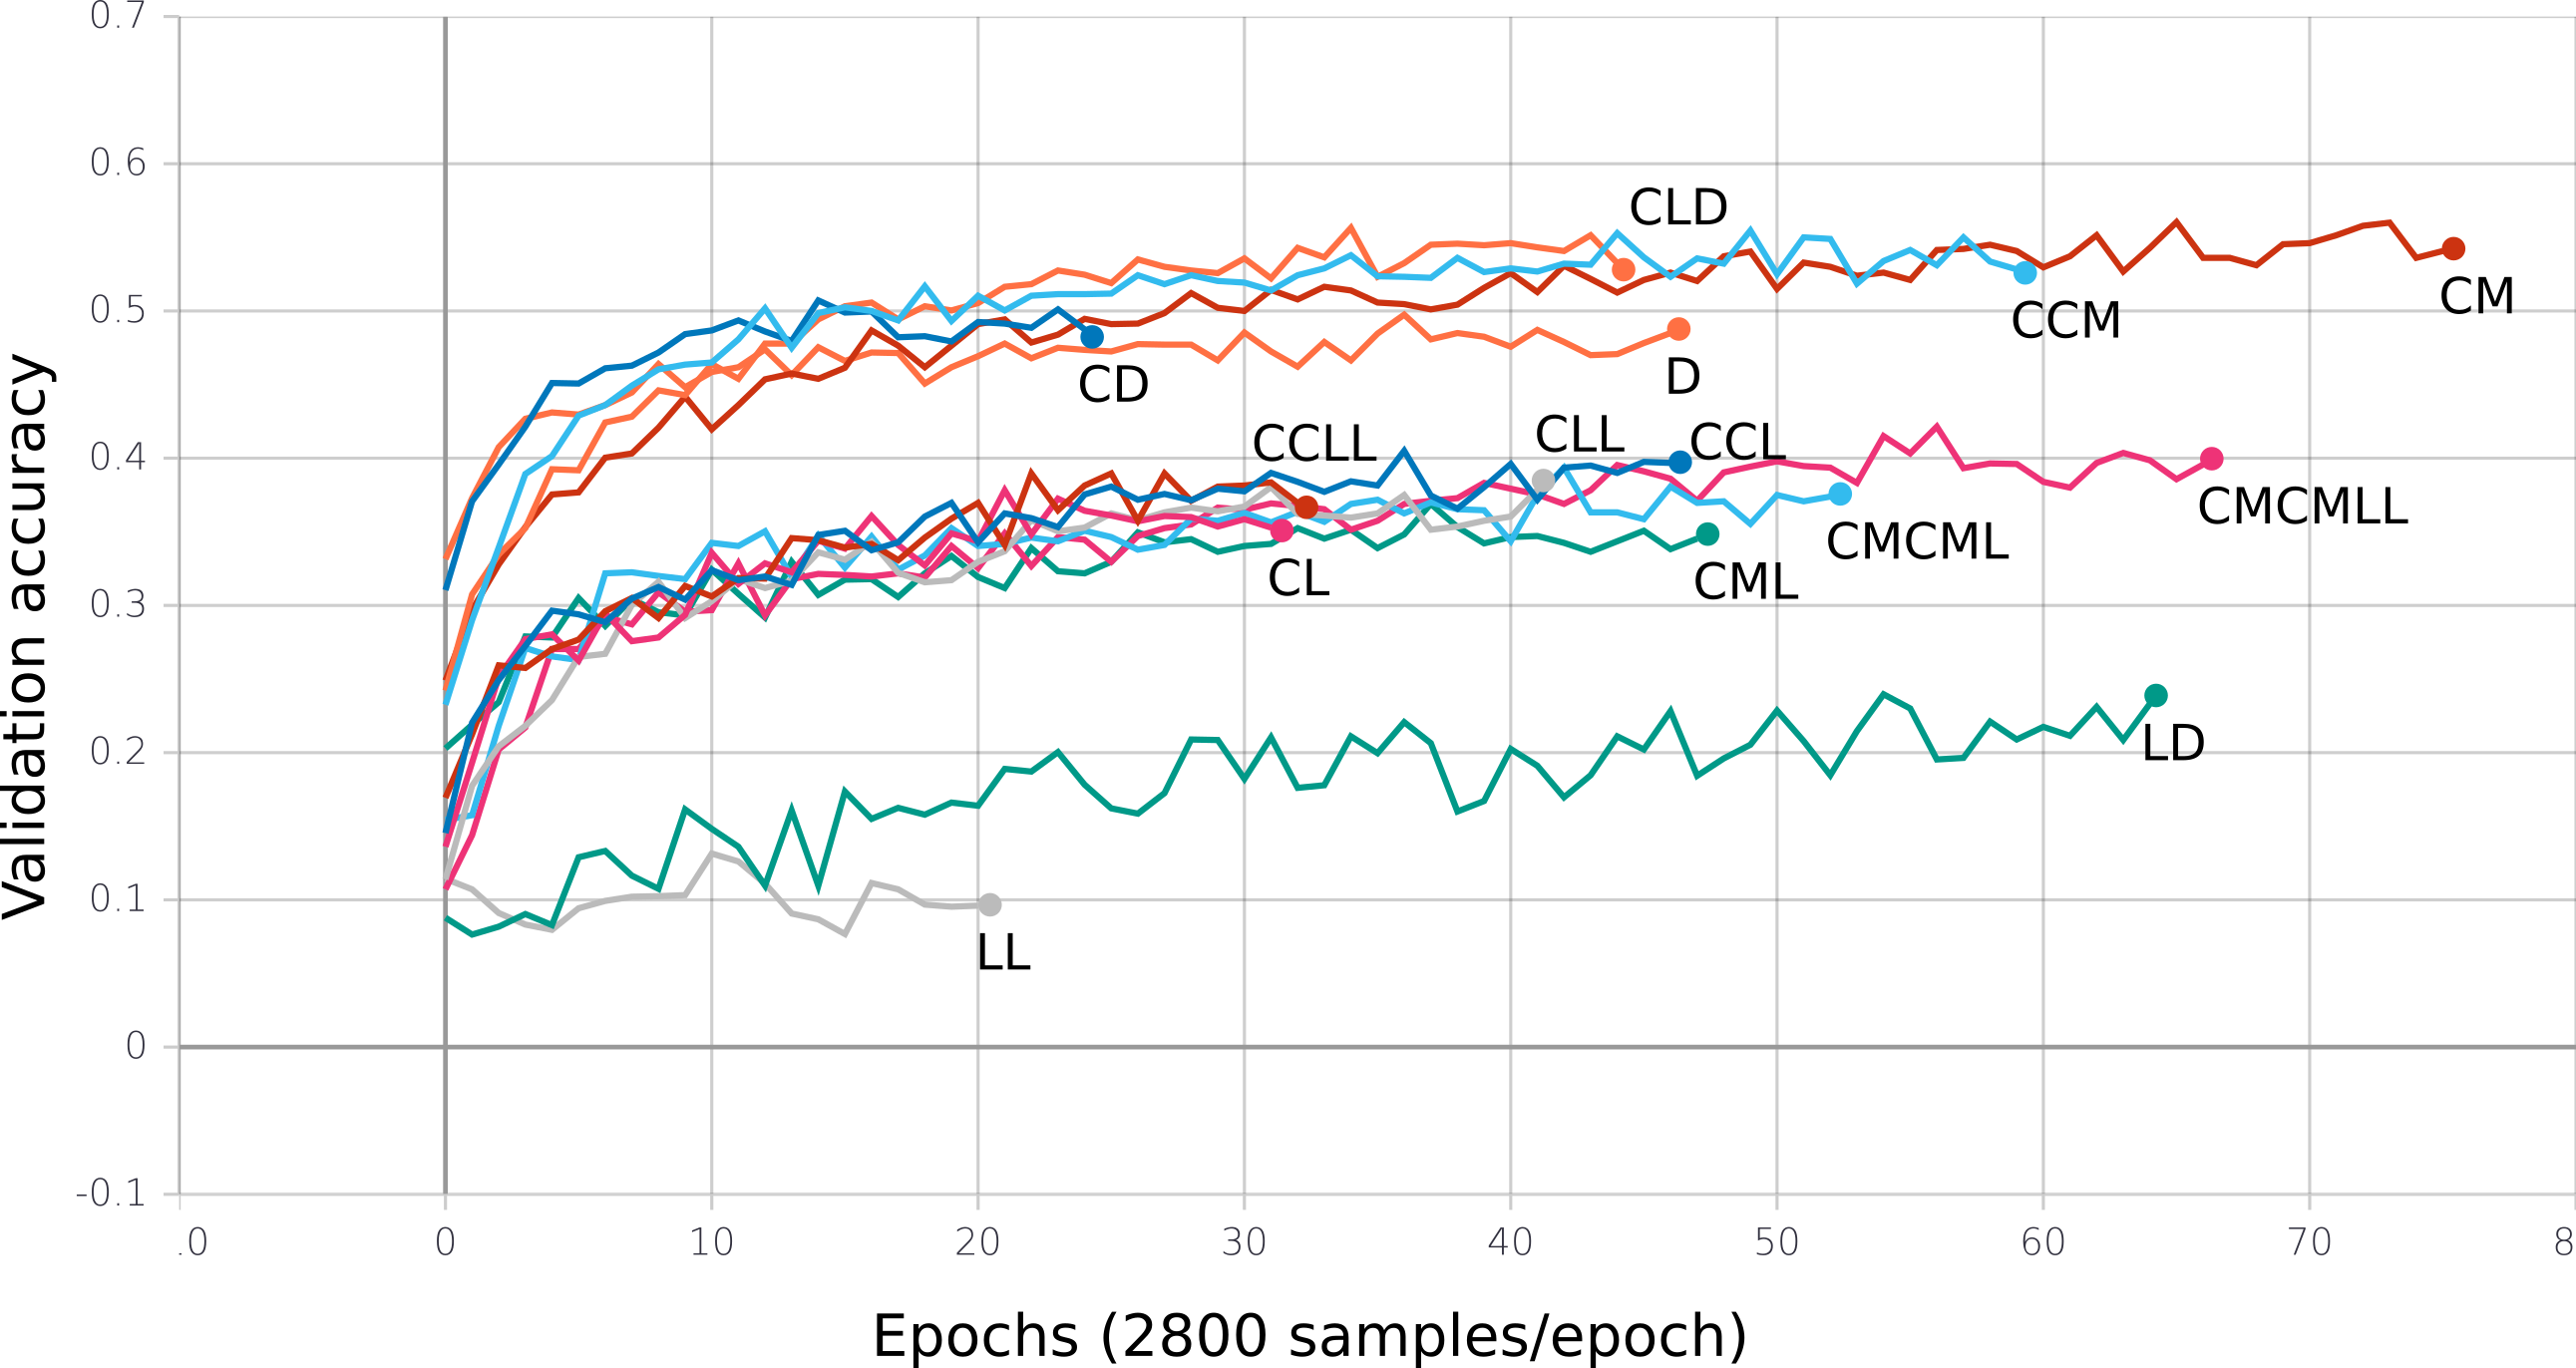
\includegraphics[width=0.9\textwidth]{content/epoch_val_categorical_accuracy.png}
\caption{\label{fig:learning}Learning curves of some models (validation accuracy vs. time)}%
\end{figure*}

%\levelB{Inputs}
%one-hot
The input features of the network for each instance is a 512x256 matrix representing only one block of 512 bytes of a random file of the dataset. Each of the 512 bytes is one-hot encoded, meaning that its value is converted into a vector with 256 elements, with only one of them set to 1, corresponding to the value of the byte, while the others are set to zero. A batch size of 100 was used, with 28 steps per epoch.

%8bits
% The input features of the network for each instance is a 512x8 matrix representing only one block of 512 bytes of a random file of the dataset. Each of the 512 bytes uses a custom encoding where each of the 8 bits of a byte is represented as -1 or 1, depending whether the bit is 0 or 1. During initial tests, this encoding was compared to three other encodings: one-hot encoding, 8 bits represented as 0 or 1\todo{include citation}, and 8 bits represented as [0,1] and [1,0] \cite{hiester_file_2018}. More research should be done in the future to determine the best of the four, but initial results suggest they have similar impact on the model accuracy. The one-hot encoding has the disadvantage of increasing the input matrix size by a factor of 32.

%\levelB{Outputs}
The output of the network for a given instance is a vector with a size equal to the number of classes, subjected to a softmax function, which applies the exponential function on the vector and then normalizes it. Each value will represent the predicted probability that the instance belongs to a specific class.

%exp18
The two models that used LSTM layers without convolutional layers presented slower learning in comparison with the others, as can be seen in figure \ref{fig:learning}. The validation accuracy values can be consulted in figure \ref{fig:models}.


\noindent
\begin{figure*}[htb!]
\centering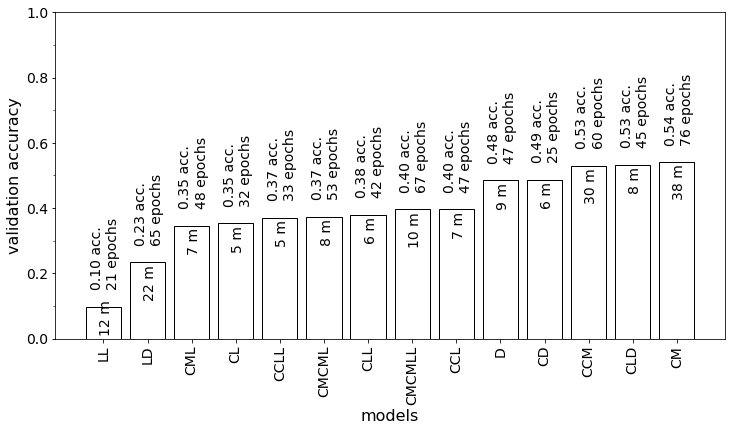
\includegraphics[width=1.0\textwidth]{content/models.png}
\caption{\label{fig:models}The bar plot shows the validation accuracy of the considered models. Their training time, in minutes, and the total epochs processed is also indicated. The training was interrupted when no further improvement was observed for 10 consecutive epochs.}%
\end{figure*}


The validation accuracy values of the remaining models were in the 0.35-0.54 range.

% The selected model for further research, identified as ``CM'', achieved an accuracy of 0.54. The models, ``CLD'' and ``CCM'' achieved similar values, but model ``CM'' performed better in the experiment described in section \ref{sec:exprandom}.

To check if the two slower models could give better results if executed for a longer period, they were trained for 10 hours. The model identified as ``LD'', which uses an LSTM layer followed by a fully connected layer, was able to achieve an accuracy of 0.494, while the other, ``LL'', achieved only 0.153.

%stagnation in learning with such short times, combined with low final accuracy suggests that the dataset present some patterns that are easily recognizable, while the rest of the dataset present a very hard classification task.

% \levelC{Limitations and threats to validity}

% \input{content/4.0.2-researchonnumberofclasses.tex}
% \input{content/4.0.3-experimentrandomdata.tex}

%     \levelB{Objective}
%     The objective of the experiments described in this section 
was to compare the accuracy level of different neural networks with a short training time constraint and using only a small training dataset, at the filetype identification task.

\todo[inline]{este é o foco do trabalho, identificação do tipo de arquivo?}

This objective should give a direct answer to the first research question ``How does different neural network models compare to each other in terms of training performance and quality of results?'', but the constraints imposed to the examined networks are related to the second question ``Which neural network models would be more suitable to accept the addition of new file types by the forensic examiners community?'', because in order to facilitate the creation of models by a community that does not necessarily will have expensive hardware, plenty of time, or extensive knowledge on neural networks, the types of networks that would be desirable to find are the ones that are fast to train.
%     \levelB{Methodology}
%     
\todo[inline]{falar da separação de primeiro bloco e todos os blocos, falar qual o tipo de resultado esperado}
\todo[inline]{qual o tipo de experimento?}
\todo[inline]{foco na identificação dos tipos de arquivos. Só isto?}
\todo[inline]{melhor descrição sobre os passos do que vai ser feito antes de descrever os experimentos}
\todo[inline]{Nos resultados, existe uma nova forma de organização, por exemplo, os primeiros blocos. Continua dizendo o que está sendo feito. Deve re-organizar (colocar na metodologia). Assim quando chegar nos experimentos e resultados o leitor já terá uma ideia geral do que será feito.}

The input features of the network for each instance is a 512x256 matrix representing only one block of 512 bytes of a random file of the dataset. Each of the 512 bytes is one-hot encoded, meaning that its value is converted into a vector with 256 elements, with only one of them set to 1, corresponding to the value of the byte, while the others are set to zero.

The output of the network for a given instance is a vector with 3 elements, subjected to a softmax function, which applies the exponential function on the vector and then normalizes it. Each value will represent the predicted probability that the instance belongs to each of the three classes, PDF, JPG or PNG.

Minimize the training time is important when the task of create new models to new filetypes is delegated to the forensic examiners community, since they may not have expensive hardware or time to train a more demanding neural network.

For similar reasons, networks that require too much tuning to perform well are undesirable, since it would require a higher knowledge and work from the forensic examiner.


%metricas
To identify networks with such requirements, each experiment use two stop conditions, ten minutes, or an accuracy of 90\% in the training set, whichever occurs first. These limits were established during the experiments.

\todo[inline]{justificar critério de parada: estabilização/estagnação; quando vai aumentando o tempo, não existia mais modificações, ou seja 10 minutos chegavam para a estabilidade do modelo}

%Since the rate of change of accuracy may present oscillations during training, a visual comparison of accuracy versus time curves is important to confirm which network has better training times.

All the experiments use the Adam \cite{kingma_adam:_2014}
optimization algorithm to guide backpropagation, which was selected because it performed well in the preliminary results without requiring tuning the learning rate.

%modelos
The networks considered used different combinations of convolutional, max pooling, LSTM, and fully connected layers.

The experiment names are based on the types of layers that compose each architecture and their purpose is to differentiate one experiment of another. Thus, they are not intended to be used outside of this work.



%     \levelB{Datasets}
%     Datasets for three different file types, JPG, PDF, and PNG, were obtained from online sources.

The PDF files were retrieved from http://arxiv.org/pdf/, which stores them using a sequential nomenclature. The training dataset uses the files 1904.10000.pdf to 1904.10099.pdf, development 1904.10100.pdf to 1904.10199.pdf, and test 1904.10200.pdf to 1904.10299.pdf. 

The JPG samples were obtained in ftp://ftp.inrialpes.fr/pub/lear/douze/data/jpg1.tar.gz  \cite{jegou_hamming_2008}, and 100 images were assigned to training, 100 to development and the remaining 612 to test.
%If you use this dataset, please cite the following paper:
% Herve Jegou, Matthijs Douze and Cordelia Schmid
% "Hamming Embedding and Weak geometry consistency for large scale image search"
% Proceedings of the 10th European conference on Computer vision, October, 2008

The PNG images were obtained from \url{http://data.vision.ee.ethz.ch/cvl/DIV2K/DIV2K_train_HR.zip} \cite{agustsson_ntire_2017}, and 100 images were assigned to training, 100 to development and the remaining 700 to test.

%dataset paper: http://www.vision.ee.ethz.ch/~timofter/publications/Agustsson-CVPRW-2017.pdf
% @InProceedings{Agustsson_2017_CVPR_Workshops,
% author = {Agustsson, Eirikur and Timofte, Radu},
% title = {NTIRE 2017 Challenge on Single Image Super-Resolution: Dataset and Study},
% booktitle = {The IEEE Conference on Computer Vision and Pattern Recognition (CVPR) Workshops},
% month = {July},
% year = {2017}
% }

%     \levelB{Environment}
%     The experiments did not take advantage of GPU acceleration and were  conducted on a single computer with 256GB of RAM and with 2 Intel\textregistered Xeon\textregistered E5-2630 v2 processors, with 6 cores each, with 2 hyper-threads per core, or 24 hyper-threads in total. 

The source code for the experiments is available at \url{http://github.com/atilaromero/ML}.



% \levelA{Results}
% 










%     \levelB{First block as input}
%     \todo[inline] {deixar mais claro antes que os experimentos estão organizados desta forma}
\todo[inline] {aumentar fonte nas bordas das figuras}

In the first set of experiments, for each file selected as input sample from the test dataset, only the first 512 bytes of that file were used. For most filetypes, including those three under consideration, these first bytes contains regular patterns in fixed positions, which makes them easy to recognize.

Each epoch was configured to draw 100 samples from the training dataset. Validation was performed using 100 samples from the development dataset. Each sample had only 512 bytes.

Three network configurations were compared. The simplest one was a feedforward network, referred as ``D'', with only a single fully connected layer, with 131072 input units (512 bytes times 256 possible values using one hot encoding) and 3 output units, one for each output class, PDF, JPG, or PNG.

Another one, referred as ``LD'', used a LSTM layer with 32 output units, followed by a fully connected layer of 3 output units. The LSTM layer process one byte per time step. This is one of the simplest LSTM configurations. While it would be possible to use only a single LSTM layer without a fully connected layer next, then the LSTM layer would have to be limited to 3 output units, and would have too few trainable parameters. 

The last one, referred as ``CL'', used a convolutional layer without max pooling with 32 input units, 3 output units, and a stride of 32 followed by a LSTM layer with 3 output units. Some other convolution sizes and strides were tried during the test development. A convolutional layer with 512 units of input would be equivalent to a fully connected layer, as no convolution would be performed. Using 32 input units and a stride of same size, the convolutional layer breaks the block in 16 parts with 32 bytes each. The convolutional layer already outputs the exact number of classes, thus the LSTM layer here is just summarizing the results.

Table \ref{tab:carving7-11} gives a summary of the results of this set of experiments, listing for each model the number of trainable parameters, if the training used all of the blocks of the sample file or just the first one, the number of training epochs, the duration of the training, and the final accuracy on the training and on the validation datasets.

\begin{table*}[!ht]
    \centering
    \caption{Filetype identification experiments with first block}
    \label{tab:carving7-11}
\begin{tabular}{r|r|r|r|r|r|r}
\hline
Name & Parameters & Blocks & Epochs & Time    & Training          & Validation          \\       
     &            &        &        &         &          accuracy &            accuracy \\ \hline\hline

D	& 393219	& first	& 1	    & 0m01s	& 0.91	& 1.0 \\ \hline
LD	& 37091	    & first	& 28	& 2m54s	& 0.92	& 0.68 \\ \hline
CL	& 24663	    & first	& 4	    & 0m05s	& 0.98	& 0.73 \\ \hline
\end{tabular}
\end{table*}

The simple feedforward network was the fastest networking concerning training time, and had the best validation accuracy. It is interesting to notice that the LSTM without a previous convolutional network had a slow training time in comparison.

Since the simplest network was giving the best results, the next experimentation step was to check if this performance would be maintained in a more complex scenario.


%     \levelB{Random block as input}
%     The next set of experiments uses a random block (512 bytes chunks) from each file, instead of just the first one. This is a harder classification task because, while in the first block is reasonable to find patterns in specific positions in relation to the beginning of the block, this correspondence is not normally preserved in the remaining blocks, as the pattern may start anywhere in the block. The second factor is that in files with low compression rates, as image files, the beginning of the file normally presents more recognizable patterns than the middle.

Each epoch was configured to draw 1000 samples from the training dataset. Validation was performed using 1000 samples from the development dataset. Each sample had only 512 bytes.

Comparing the three network structures used in the previous set of experiments, the ``CL'' network had the best results.
%12 D
The simple feedforward network, ``D'', that performed well classifying the first block was unable to achieve similar results when classifying a random block.

%LD
The network using only a LSTM layer followed by a fully connected layer, ``LD'', was the slowest to train, and achieved a low accuracy when compared to the other two networks.

%CL
The network ``CL'', that used a convolutional layer to divide the input block in 16 smaller blocks of 32 bytes and used the LSTM layer to process the results gave best results of the three.

\begin{table*}[!ht]
    \centering
    \caption{Filetype identification experiments with random block}
    \label{tab:carvingrandomblock}
\begin{tabular}{r|r|r|r|r|r|r}
\hline
Name & Parameters & Blocks & Epochs & Time    & Training          & Validation          \\       
     &            &        &        &         &          accuracy &            accuracy \\ \hline\hline

D       & 393219    & all   & 282   & 10m01s    & 0.764 & 0.719 \\\hline
LD      & 37091     & all   & 10    & 10m35s    & 0.559 & 0.365 \\\hline
CL      & 24663     & all   & 159   & 10m00s    & 0.83  & 0.789 \\\hline
\end{tabular}
\end{table*}

\noindent
\begin{figure*}[htb!]
\centering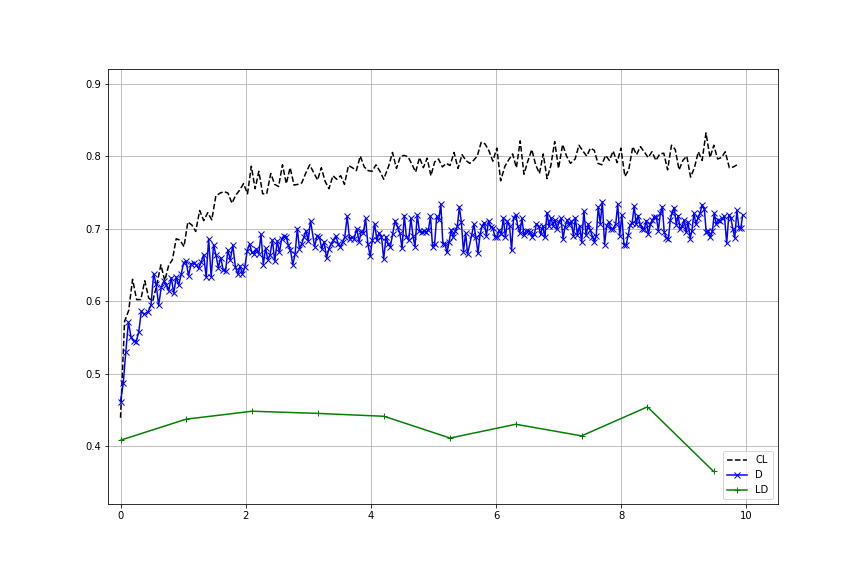
\includegraphics[width=0.50\textwidth]{content/CL-D-LD.png}
\caption[Experiments with random blocks]{\label{fig:randomblock}Filetype identification experiments with random block - validation accuracy vs. time(minutes)}%
\end{figure*}

%     \levelB{CL variations}
%     
Three variations of the ``CL'' network were made.
The ``CML'' network simply adds a max pooling layer to the convolutional layer.

The ``CLL'' network increases the output units of the convolutional layer and adds a LSTM layer with 64 output units before the final LSTM layer with 3 outputs. This change gives more parameters to the LSTM part of the network.

The ``CLD'' network also tries to increase the influence of the LSTM layer in the network. It reduces the convolutional input window while increases the number of output units. The number of output units of the LSTM network is increased to 128 and a fully connected layer is used as output layer.

The results of the experiments with these variations is shown in table \ref{tab:carvingclvariations}.
Overall, this three variations produced better results than the ``CL'' network, as can be seen in figure \ref{fig:cl-variations}.

\begin{table*}[!ht]
    \centering
    \caption[CL variations]{Comparison of models that use convolutional layers and LSTM layers}
    \label{tab:carvingclvariations}
\begin{tabular}{r|r|r|r|r|r|r}
\hline
Name & Parameters & Blocks & Epochs & Time    & Training          & Validation          \\       
     &            &        &        &         &          accuracy &            accuracy \\ \hline\hline

CL      & 24663     & all   & 159   & 10m00s    & 0.83  & 0.789 \\\hline
CLL     & 287824    & all   & 108   & 10m04s    & 0.879 & 0.856 \\\hline
CML     & 262416    & all   & 137   & 10m03s    & 0.863 & 0.836 \\\hline
CLD     & 1246339   & all   & 73    & 8m48s     & 0.902 & 0.857 \\\hline
\end{tabular}
\end{table*}

\noindent
\begin{figure}[htb!]
\centering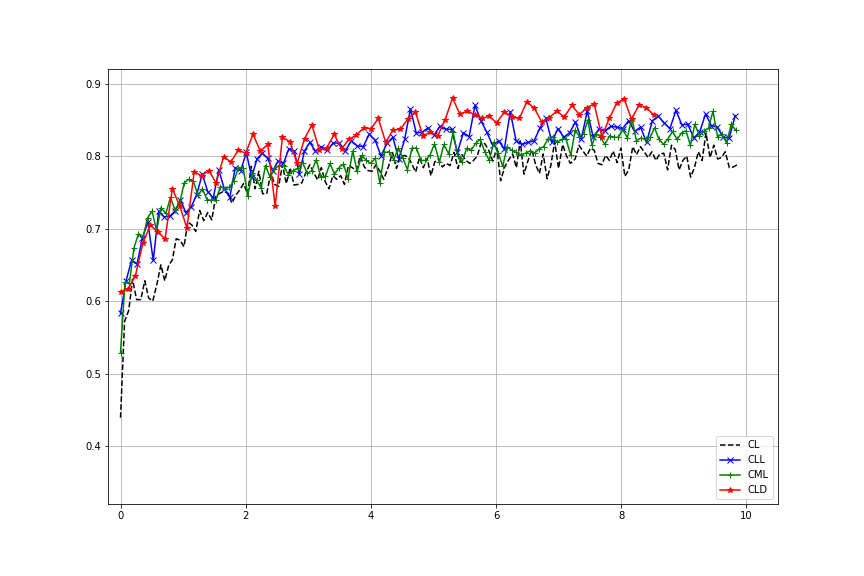
\includegraphics[width=0.50\textwidth]{content/CL-CLL-CML-CLD.png}
\caption[CL variations]{\label{fig:cl-variations}Comparison of models that use convolutional layers and LSTM layers - validation accuracy vs. time(minutes)}%
\end{figure}

%     \levelB{No LSTM}
%     To test if 
the LSTM layer could be replaced by 
another way of aggregating the convolutional layer outputs, three networks were constructed without any LSTM layer.

One of them, ``CM'' uses a stride of one and aggregates the results using a big max pooling layer.

Another one, ``CCM'' uses the same strategy, but includes another convolutional layer before the max pooling.

The last one, ``CD'', uses a bigger input window of 64 units, but with a smaller stride of 8 units. The output layer is a fully connected layer.

The results are shown in table \ref{tab:carvingnolstm}. The ``CL'' network is included for comparison.
These three networks produced similar results, but they are not as good as the ``CL'' network, as can be seen in figure
\ref{fig:nolstm}.


\begin{table*}[!ht]
    \centering
    \caption[No LSTM]{Comparison of models that do not use LSTM}
    \label{tab:carvingnolstm}
\begin{tabular}{r|r|r|r|r|r|r}
\hline
Name & Parameters & Blocks & Epochs & Time & Training          & Validation          \\       
     &            &        &        &         &          accuracy &            accuracy \\ \hline\hline

CL      & 24663     & all   & 159   & 10m00s    & 0.83  & 0.789 \\\hline
CM      & 24579     & all   & 98    & 10m01s    & 0.806 & 0.796 \\\hline
CCM     & 24600     & all   & 93    & 10m04s    & 0.778 & 0.786 \\\hline
CD      & 1059587   & all   & 144   & 10m00s    & 0.758 & 0.751 \\\hline
\end{tabular}
\end{table*}

\begin{figure}[htb!]
\centering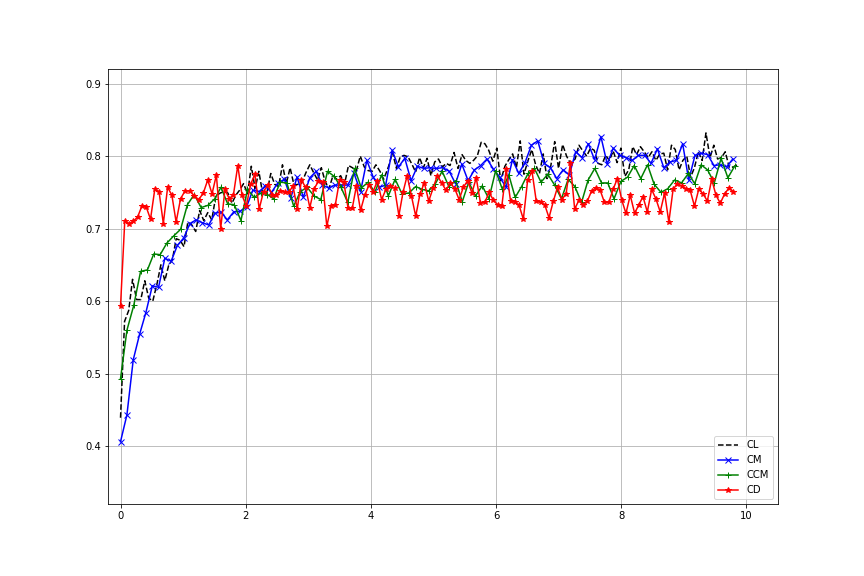
\includegraphics[width=0.50\textwidth]{content/CL-CM-CCM-CD.png}
\caption[No LSTM]{\label{fig:nolstm}Comparison of models that do not use LSTM - validation accuracy vs. time(minutes)}%
\end{figure}


%     \levelB{Two convolutional layers}
%     To test if an increase on the deepness of the network would improve its results, four networks using two convolutional layers were experimented. 

At the ``CCL'' network, the first convolutional layer uses 8 units for the input window, and a stride of the same size, thus dividing the 512 bytes of the input block in 64 matrices of 8x256 that are then converted in 64 vectors of 128 units. The second layer divides the 64x128 input in 8 matrices of 8x128, producing 8 vectors of 64 units. The LSTM layer uses each of these 8 vectors as time steps, producing a single vector of 3 units, one for each class.

The ``CCLL'' network adds a LSTM layer of 64 output units between the convolutional layers and the final LSTM layer.

The ``CMCML'' network is similar to ``CCL'', but uses max pooling of size 2 at each convolutional layer. This max pooling act on the second dimension instead of the first, and thus does not change the number of steps that the LSTM layer will process. For example, the first max pooling halves the number of output units of the first convolutional layer from 128 to 64.

The ``CMCMLL'' network combines the two additions, using max pooling and using two LSTM layers.

The results are shown in table \ref{tab:carving2convs}. The ``CL'' network is included for comparison. The  ``CL'' network results were only better than the the ``CCL'' network. The other three networks presented better accuracy values, as can be seen in figure \ref{fig:nolstm}.The ``CMCML'' and ``CMCMLL'' results were similar.

\begin{table*}[!ht]
    \centering
    \caption[Two convolutional layers]{Comparison of models that use two convolutional layers}
    \label{tab:carving2convs}
\begin{tabular}{r|r|r|r|r|r|r}
\hline
Name & Parameters & Blocks & Epochs & Time & Training          & Validation          \\       
     &            &        &        &         &          accuracy &            accuracy \\ \hline\hline

CL      & 24663     & all   & 159   & 10m00s    & 0.83  & 0.789 \\\hline
CCL     & 328688    & all   & 171   & 10m00s    & 0.793 & 0.752 \\\hline
CCLL    & 361712    & all   & 153   & 10m00s    & 0.821 & 0.84  \\\hline
CMCML   & 295536    & all   & 107   & 6m30s     & 0.901 & 0.873 \\\hline
CMCMLL  & 320752    & all   & 102   & 7m30s     & 0.904 & 0.892 \\\hline
\end{tabular}
\end{table*}

\begin{figure}[htb!]
\centering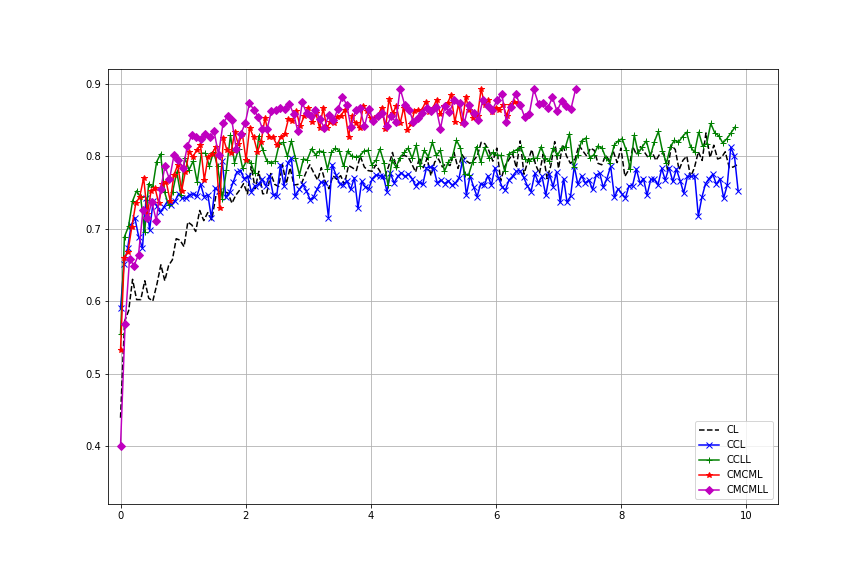
\includegraphics[width=0.50\textwidth]{content/CL-CCL-CCLL-CMCML-CMCMLL.png}
\caption[Two convolutional layers]{\label{fig:twoconvs}Comparison of models that use two convolutional layers - validation accuracy vs. time(minutes)}
\end{figure}


%     \levelB{Discussion}
%     The best networks found among those examined in all set of experiments are the ``CLD'', ``CMCML'' and ``CMCMLL''. They have similar training times and final accuracy results. Their accuracy curves are shown in figure \ref{fig:bestnets}.

\begin{figure}[htb!]
\centering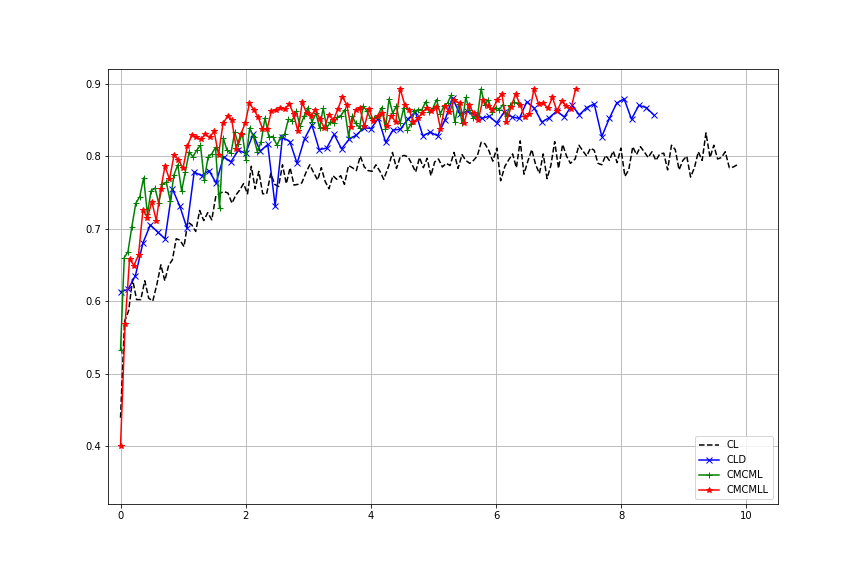
\includegraphics[width=0.50\textwidth]{content/CL-CLD-CMCML-CMCMLL.png}
\caption[Best networks]{\label{fig:bestnets}Three networks with best accuracy - validation accuracy vs. time(minutes)}
\end{figure}

While a simple feedforward network worked well to classify the beginning of a file, there are better options to classify a block sample taken from the middle of the file.

The convolutional and LSTM layers worked well together, better than either one in isolation.

Table \ref{tab:carvinglayers} specify the number of output units in each layer of the networks used in the experiments. For the networks with two convolutional layers, those layers are connected together before the LSTM layer. For the convolutional layers, the input number indicates the size of the receptive field. 
\begin{table*}[!ht]
    \centering
    \caption{Experiments layers}
    \label{tab:carvinglayers}
\begin{tabular}{r|r|r|r|r|r|r}

       & \multicolumn{4}{|c|}{}                         &        & Fully           \\     
       & \multicolumn{4}{|c|}{Convolutional}            & LSTM   &       connected \\ \hline
Name   & Input         & Stride & Output & Pooling size & Output & Output          \\ \hline\hline

D      &               &        &        &              &        & 3               \\ \hline
LD     &               &        &        &              & 32     & 3               \\ \hline
CL     & 32            & 32     & 3      &              & 3      &                 \\ \hline
\hline
CLL    & 32            & 32     & 32     &              & 64     &                 \\       
       &               &        &        &              & 3      &                 \\ \hline
CML    & 32            & 32     & 32     & 2            & 3      &                 \\ \hline
CLD    & 16            & 16     & 256    &              & 128    & 3               \\ \hline
\hline
CM     & 32            & 1      & 3      & 481          &        &                 \\ \hline
CCM    & 32            & 1      & 3      &              &        &                 \\       
       & 2             & 2      & 3      & 240          &        &                 \\ \hline
CD     & 64            & 8      & 64     &              &        & 3               \\ \hline
\hline
CCL    & 8             & 8      & 128    &              & 3      &                 \\       
       & 8             & 8      & 64     &              &        &                 \\ \hline
CCLL   & 8             & 8      & 128    &              & 64     &                 \\       
       & 8             & 8      & 64     &              & 3      &                 \\ \hline

CMCML  & 8             & 8      & 128    & 2            & 3      &                 \\       
       & 8             & 8      & 64     & 2            &        &                 \\ \hline
CMCMLL & 8             & 8      & 128    & 2            & 64     &                 \\       
       & 8             & 8      & 64     & 2            & 3      &                 \\ \hline

\end{tabular}
\end{table*}

The fact that it was possible to distinguish between JPG and PNG file blocks shows the potential of neural networks to perform data carving, as this filetypes have compression and therefore should present few recognizable structures. The PDF file format introduces another type of challenge, as it can enclose the other two filetypes. 

%5
\levelA{\label{chap:conclusion}Discussion of results}
The results may be grouped in three groups. The models that used LSTM without a convolutional layer performed poorly. The models with convolutional layers that used LSTM as the final layer had intermediary results. The remaining models were the single layer perceptron (single fully-connected layer model, identified as ``D'') and the models that used convolutional models and used a fully-connected layer or maxpooling as the last layer.

The best accuracy results were from the three models identified as ``CCM'', ``CM'', and ``CLD'', but the latter had faster training time and also showed good resilience to changes: during preliminary tests and later when test conditions where altered to try to improve results, this model and its variations always were among the best models while the others were not.

In this research, the models were not trained until exhaustion. This was initially done to identify which models would be most promising for future testing, but further attempts to tune layer types, quantity and parameters resulted in accuracy values still close to 0.54, which suggests that selection or tuning of models may not be the best approach to improve results.


% Among the examined networks, while some of them satisfy the requirements imposed and could potentially be used by a forensic examiner to create a model to a new file type, the networks that showed the best results are those that use convolutional layers to split and process the input and then use LSTM layers to analyse the series of outputs produced by the convolutional layers. This gives a direct answer to the first research question, ``How does different neural network models compare to each other in terms of training performance and quality of results?''.

% To answer the second question, ``Which neural network models would be more suitable to accept the addition of new filetypes by the forensic examiners community?'', a set of constraints were imposed to the analyzed models. The achieved results can be replicated with little computational power, in a short time period and with limited datasets.

% To create models that recognize new filetypes, a forensic examiner would have to gather a small dataset for each filetype that needs to be recognized. Datasets of 100 files were sufficient to run the experiments in this work, but it is possible that even smaller datasets could be used. Then, a network with two convolutional layers with max pooling followed by a LSTM layer could be used to quickly train a new model, without the requirement of special hardware. In the chosen framework, Keras, the export and import of models can be easily done, so the forensic examiner could export and publish the new model in a public repository.


    \levelB{Future work}
    The models required short training times and few examples to approach their limit.
This suggests that some patterns were very easy to find but they were insufficient to achieve a higher accuracy.
This raises the question whether there are harder patterns that could be found by a better model not yet tried or if this a more fundamental issue that would not be solved by a trial and error approach of tweaking of parameters and layer modifications.

Based on the work presented here, further studies focused on error analysis are in progress to address this question.

%  For future researches on file fragment classification, the hypothesis that the remaining 2/3 of the observed errors are caused by similar data structures used by multiple files should be explored. Also, the search for a procedure to automatically label inner data structures of files may be a promising strategy. 

% Having recognized the potential of neural networks in the data carving task, there are still some research paths that should be explored.

% \todo[inline]{qual a dificuldade da tarefa de identificacao do tipo de arquivo, o que os outros metodos atingem de acuracia?}

% \todo[inline]{aumentar número de tipos de arquivos suportados}

% \todo[inline]{Existem aspectos que já avançaram mas não citados no texto, por exemplo, já consegue identificar o início e o fim do arquivo.}

% One of them is about the increase in the range of supported filetypes. In a collaborative approach, should the said community be sharing models, datasets, or both? What are the strengths and weakness of each?

% Another one is about reassembling. After each block has been classified, how to reconstruct the original file in the occurrence of fragmentation?

% \todo[inline]{Quanto a remontagem? Existe uma previsão e qual o dataset tu vais utilizar? Como vai conseguir remontar? Este problema é complicado, mas deve tentar avançar de alguma forma.}

% \todo[inline]{Pretende ainda avançar nos tipos de arquivos e na remontagem. Mesmo que não consiga remontar, pelo menos mostrar o que não conseguiu, pois facilita para quem for feito. —> Verificar a literatura se ninguém está fazendo isto mesmo.}

% The last one is about the recognized structures. Is it possible to use the trained networks to describe the structures being recognized?

% ==========


% The following questions are intended to be answered in future works: 

% \begin{enumerate}[itemindent=\parindent,label=\textbf{Q\arabic*.}]

%     \item Could a neural network based tool support a wider range of file types?
    
%     \item Could a neural network based tool handle fragmentation through reassembling?
    
%     % \item Do the results obtained with usual datasets reflect what happens in real scenarios?

% \item Do neural networks help to interpret internal file structures?

% \end{enumerate}

% \todo[inline]{compare solutions - possible candidates: feedforward, convolutional, LSTM, BLSTM, SVM, kNN, Photorec, Foremost, scalpel}
% \todo[inline]{shuffle data to simulate fragmentation}
% \todo[inline]{removal of portions of files to simulate data corruption}
% \todo[inline]{increase the number of supported file types, investigating the best strategy to scale the solution}
% \todo[inline]{reassembling}
% \todo[inline]{model share}
% \todo[inline]{adaption of visualization techniques of neural networks, attempting to infer file structure.}

\levelA{Conclusion}
This study evaluates some alternative models in the file fragment classification task. The expectation was to identify the most promising models for improvement. But an apparent limit was found on how far these models could be improved.

% Using different combinations of layers and parameters, the expectation was that some models would be discarded and some would be selected as promising alternatives. That could be used to guide future researches and also serve as a reference for comparison between studies. 
The Govdocs1 dataset brought an important basis for comparison to be used between carving solutions. But to achieve easily reproducible results, the models must also be publicly available, a condition not all revised studies fulfill. Being available as Jupyter notebooks at https://github.com/atilaromero/carving-experiments, the results described here should require little effort to be reproduced. Thus the models presented here can be used as a basis of comparison in  future researches.

